\documentclass{standalone}
%outline around text
\usepackage[outline]{contour}
\contourlength{1.3pt}

%tikz
\usepackage{tikz}
\usetikzlibrary{knots, cd, calc}

\begin{document}



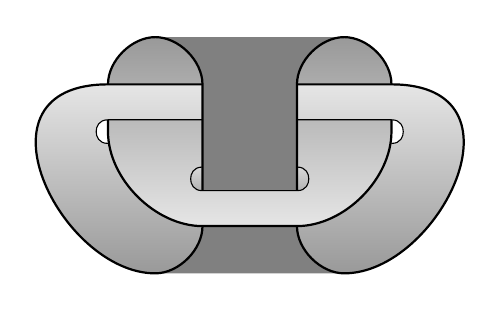
\begin{tikzpicture}[scale=0.6]
\clip (-4.7, -0.2) rectangle (4.7, 5.2);
\fill[%pattern = north west lines
		color = black!50]
	(-2, 5) -- 
	(2, 5) .. controls +(-0.5, 0) and +(0, 0.5) ..
	(1, 4) -- 
	(1, 1) .. controls +(0, -0.5) and +(-0.5, 0) ..
	(2, 0) --
	(-2, 0) .. controls +(0.5, 0) and +(0, -0.5) ..
	(-1, 1) --
	(-1, 4) .. controls +(0, 0.5) and +(0.5, 0) ..
	(-2, 5);
	
\fill[top color = black!40, bottom color = black!10] 
	(-2, 5) .. controls +(-0.5, 0) and +(0, 0.5) ..
	(-3, 4) --
	(-3, 3) .. controls +(0, -1) and +(-1, 0) ..
	(-1, 1) -- 
	(1, 1) .. controls +(1, 0) and +(0, -1) ..
	(3, 3) -- 
	(3, 4) .. controls +(0, 0.5) and +(0.5, 0) ..
	(2, 5) .. controls +(-0.5, 0) and +(0, 0.5) ..
	(1, 4) --
	(1, 1.75) --
	(-1, 1.75) --
	(-1, 4) .. controls +(0, 0.5) and +(0.5, 0) ..
	(-2, 5);
	
\fill[bottom color = black!40, top color = black!10]
	(2, 0) .. controls +(2, 0) and +(3, 0) ..
	(3, 4) -- 
	(1, 4) --
	(1, 3.25) --
	(3, 3.25) --
	(3, 3) .. controls +(0, -1) and +(1, 0) ..
	(1, 1) .. controls +(0, -0.5) and +(-0.5, 0) ..
	(2, 0);
	
\fill[bottom color = black!40, top color = black!10]
	(-2, 0) .. controls +(-2, 0) and +(-3, 0) ..
	(-3, 4) -- 
	(-1, 4) --
	(-1, 3.25) --
	(-3, 3.25) --
	(-3, 3) .. controls +(0, -1) and +(-1, 0) ..
	(-1, 1) .. controls +(0, -0.5) and +(0.5, 0) ..
	(-2, 0);

\fill[bottom color=black!30, top color=black!15] 
	(-1, 2.25) .. controls +(-0.2, 0) and +(0, 0.1) ..
	(-1.25, 2) .. controls +(0, -0.1) and +(-0.2, 0) ..
	(-1, 1.75) -- (-1, 2.25);
\fill[bottom color=black!30, top color=black!15]
	(1, 1.75) .. controls +(0.2, 0) and +(0, -0.1) ..
	(1.25, 2) .. controls +(0, 0.1) and +(0.2, 0) ..
	(1, 2.25) -- (1, 1.75);	
	
	
	
\fill[color=white]
	(-3, 3.25) .. controls +(-0.2, 0) and +(0, 0.1) ..
	(-3.25, 3) .. controls +(0, -0.1) and +(-0.2, 0) ..
	(-3, 2.75);
\fill[color=white]
	(3, 3.25) .. controls +(0.2, 0) and +(0, 0.1) ..
	(3.25, 3) .. controls +(0, -0.1) and +(0.2, 0) ..
	(3, 2.75);
	
	
\draw (-1, 2.25) .. controls +(-0.2, 0) and +(0, 0.1) ..
	(-1.25, 2) .. controls +(0, -0.1) and +(-0.2, 0) ..
	(-1, 1.75) -- 
	(1, 1.75) .. controls +(0.2, 0) and +(0, -0.1) ..
	(1.25, 2) .. controls +(0, 0.1) and +(0.2, 0) ..
	(1, 2.25);

\draw (-1, 3.25) -- 
	(-3, 3.25) .. controls +(-0.2, 0) and +(0, 0.1) ..
	(-3.25, 3) .. controls +(0, -0.1) and +(-0.2, 0) ..
	(-3, 2.75);
\draw (1, 3.25) -- 
	(3, 3.25) .. controls +(0.2, 0) and +(0, 0.1) ..
	(3.25, 3) .. controls +(0, -0.1) and +(0.2, 0) ..
	(3, 2.75);
	
\draw[thick] (1, 1) .. controls +(0, -0.5) and +(-0.5, 0) ..
	(2, 0) .. controls +(2, 0) and +(3, 0) ..
	(3, 4) --
	(1, 4);
	
\draw[thick] (-1, 1) .. controls +(0, -0.5) and +(0.5, 0) ..
	(-2, 0) .. controls +(-2, 0) and +(-3, 0) ..
	(-3, 4) --
	(-1, 4);
	
\draw[thick] (-3, 3.25) -- (-3, 3) .. controls +(0, -1) and +(-1, 0) ..
	(-1, 1) -- 
	(1, 1)  .. controls +(1, 0) and +(0, -1) ..
	(3, 3) -- (3, 3.25);
	
\draw[thick] (-3, 4) .. controls +(0, 0.5) and +(-0.5, 0) ..
	(-2, 5) .. controls +(0.5, 0) and +(0, 0.5) ..
	(-1, 4) --
	(-1, 1.75);
	
\draw[thick] (3, 4) .. controls +(0, 0.5) and +(0.5, 0) ..
	(2, 5) .. controls +(-0.5, 0) and +(0, 0.5) ..
	(1, 4) --
	(1, 1.75);


\end{tikzpicture}
\end{document}
